\chapter{Stand der Technik}
Am Institut für Messtechnik wird der Einsatz von adaptiven Optiken in Messsystemen zur Wellenfrontentzerrung untersucht. 

Es wurde bereits ein Laser-Doppler-Velocimetry-Messsystem (LDV) aufgebaut, bei dem die beiden Teilstrahlen durch adaptive Optiken korrigiert werden. 

\section{Wellenfrontkorrektursysteme}
In der Lasermesstechnik kann es durch verschiedenste Einflussfaktoren zu ungewollten Verzerrung der Wellenfront kommen, die erheblich die Messunsicherheit erhöhen bzw. eine Messung ganz verhindern können. Bei der Wellenfrontkorrektur werden eben diese Verzerrungen über einen Sensor vermessen und mittels eines Regelkreises und einer adaptiven Optik korrigiert. Abb. zeigt einen möglichen Aufbau eines solchen Systems und verdeutlicht den Wellenverlauf.

\section{Particle Image Velocimetry}  
PIV ist ein berührungsloses optisches Verfahren zur Bestimmung von Geschwindigkeitsfeldern. Mithilfe von 2 in festem Zeitabstand aufgenommenen Bildern, wird der Versatz der Partikel bestimmt. Über den Quotient aus Positionsversatz und Zeitdifferenz zwischen den Bildern, kann auf die Geschwindigkeit geschlossen werden.

\begin{center}
	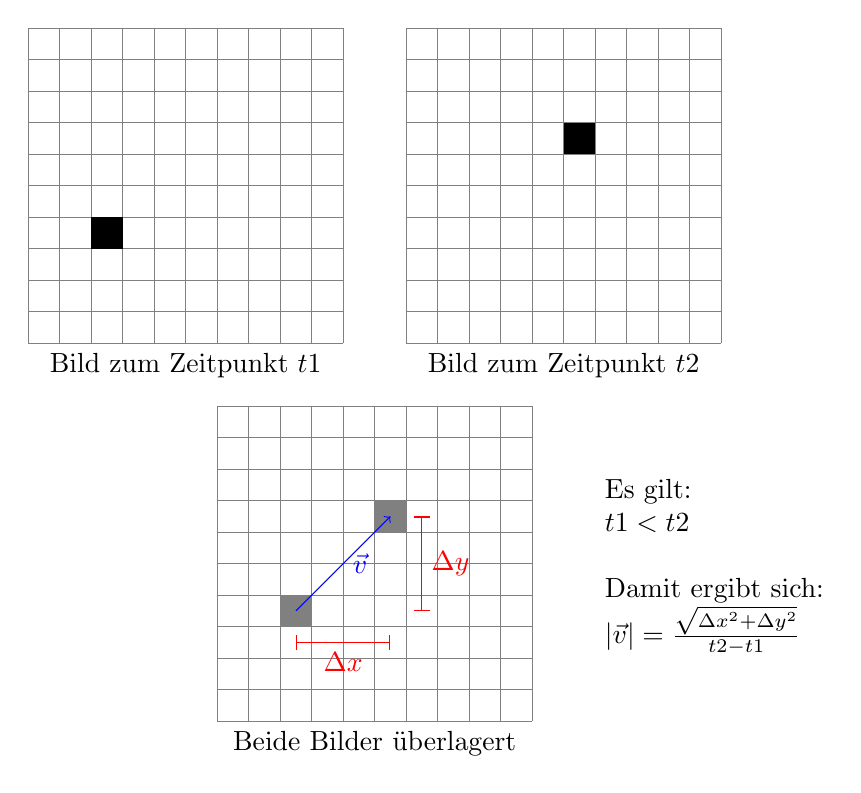
\begin{tikzpicture} [scale=0.4]
		\draw[gray] (0,0) grid (10,10);
		\draw[gray] (12,0) grid (22,10);
		
		\fill(2,3) rectangle (3,4);
		\fill(17,6) rectangle (18,7);
		
		\node[below] at (5,0) {Bild zum Zeitpunkt $t1$};
		\node[below] at (17,0) {Bild zum Zeitpunkt $t2$};
			
		\draw[gray] (6,-12) grid (16,-2);
		\node[below] at (11,-12) {Beide Bilder überlagert};
		\fill[gray](8,-9) rectangle (9,-8);
		\fill[gray](11,-6) rectangle (12,-5);
		
		\draw[|-|,red] (8.5,-9.5)--node [below]{$\Delta x$} (11.5,-9.5);	
		\draw[|-|,red] (12.5,-8.5)--node [right]{$\Delta y$} (12.5,-5.5);
		\draw[->,blue] (8.5,-8.5)--node [right]{$\vec{v}$}(11.5,-5.5);
		%\node[right] at (18,-5){Es gilt: $t1 < t2$ };
		%\node[right] at (18,-7){Damit ergibt sich: $|\vec{v}|=\frac{\sqrt{\Delta{x}^2 + \Delta{y}^2}}{t2-t1}$};
		
		\node[below right, align=left] at (18,-4){
		Es gilt:\\$t1 < t2$\\ \\
		Damit ergibt sich:\\ $|\vec{v}|=\frac{\sqrt{\Delta{x}^2 + \Delta{y}^2}}{t2-t1}$};
	\end{tikzpicture}
\end{center}


